\chapter{Описание базовой модели прямохождения робота}\label{ch:ch3}
В качестве базового алгоритма используется физическая модель, которая по заранее заданной последовательности положения стоп рассчитывает положения сервомоторов. Для уменьшения количества степеней свободы допускается ограничение на стопы – они должны быть параллельны земле всё время. Положение стоп описывается цикличным изменением следующих состояний (рисунок ~\cref{fig:base_walk_example-2}):
\begin{itemize}
  \item Обе ноги на земле, правая впереди
  \item Правая нога на земле, левая в воздухе
  \item Обе ноги на земле, левая впереди
  \item Левая нога на земле, правая в воздухе
\end{itemize}

Положение стоп в воздухе однозначно задаётся по последовательности положений стоп на земле $\{(x_i, y_i, \theta_i)\}_{i=0}^{n}$, где $x, y\in \mathbb{R}$ и $\theta \in [-\pi, \pi]$~--- положения стопы относительно изначального положения робота. Также перед исполнением алгоритма задаётся параметр $H_{step}$~--- он описывает высоту подъема стоп, и $T_{step}$~--- время совершения полного шага одной ноги в секундах. Для однозначности рассматриваются походки, которые начинаются с правой ноги, соответственное $(x_i, y_i, \theta_i)$ при чётном $i$ соответствуют положению правой ноги, а при нечётном~--- левой.

Каждая стопа на $i$-ом шаге осуществляет движение по дуге параболы, соединяющей точки $(x_i, y_i)$ и $(x_{i-2}, y_{i-2})$ с заданной высотой $H_{step}$. Так как время в задаче дискретно, то дуга также дискретизируется. В итоге порождается $\frac{T}{\tau}$ значений положений стопы $(x_i(t), y_i(t), h_i(t), \theta_i(t))$, где $t \in \{\tau, 2\tau, \cdots, T\}$. Стоит подчеркнуть, что добавляется параметр $h_i(t)$, так как стопа в промежуточных состояниях находится над воздухом.

В предположении, что одна стопа находится на земле в положении $(x_i, y_i, \theta_i)$, а вторая в положении $((x_{i+1}(t), y_{i+1}(t), \theta_{i+1}(t)))$, и обе горизонтально, а туловище вертикально, можно восстановить положение сервомоторов, чтобы достичь заданых положений \cite{inverse_1995}.

По определению этой походки можно понять, что она никак не учитывает состояние внешней среды. А последовательность передаваемых действий моделью циклична и неизменяема. Это приводит к проблемам с устойчивостью.

Любая неровность на поверхности может нарушить предположение параллельности стопы поверхности земли, а так как это главное свойство модели, то в итоге это может привести к падению робота, который продолжит совершать движения ногами без изменения модели поведения.


\begin{figure}[ht]
    \centerfloat{
        \hfill
        \subcaptionbox[List-of-Figures entry]{Обе стопы на земле, левая впереди\label{fig:base_walk_example-1}}{%
            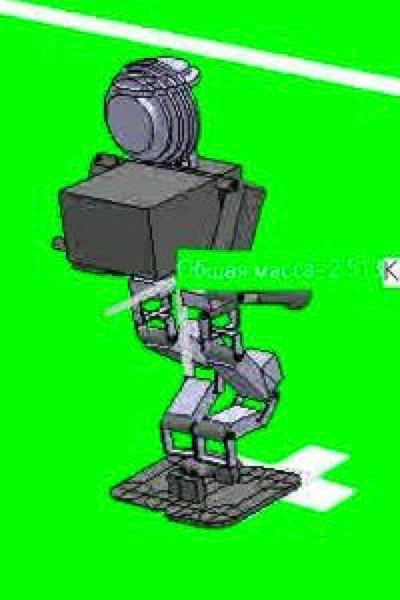
\includegraphics[width=0.3\linewidth]{images/base_walk_01.jpg}}
        \hfill
        \subcaptionbox{Правая стопа в воздухе \label{fig:base_walk_example-2}}{%
            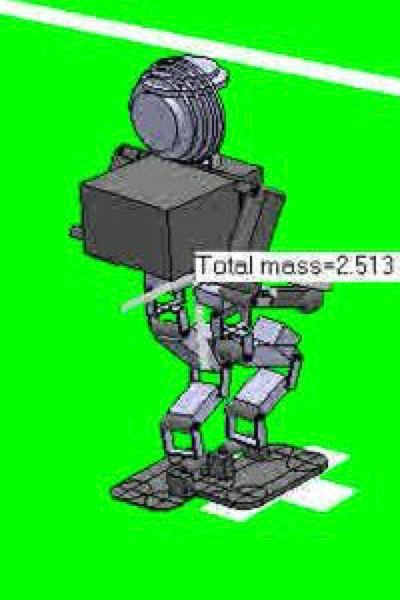
\includegraphics[width=0.3\linewidth]{images/base_walk_02.jpg}}
        \hfill
        \subcaptionbox[List-of-Figures entry]{Обе стопы на земле, правая впереди\label{fig:base_walk_example-3}}{%
            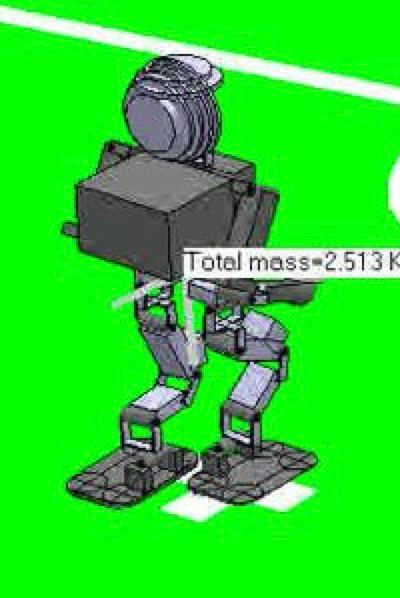
\includegraphics[width=0.3\linewidth]{images/base_walk_03.jpg}}
        \hfill
    }
    \caption[Базовая походка]{Базовая походка}\label{fig:base_walk_example}
\end{figure}
